\documentclass[tikz,border=2mm]{standalone} 
\usetikzlibrary{positioning, arrows, tikzmark}


\begin{document}
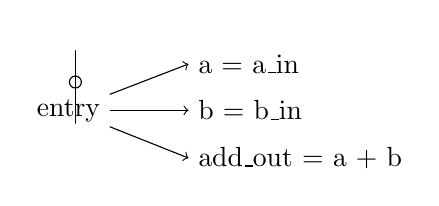
\begin{tikzpicture}[remember picture]
    \node (add-entry) {entry};
    \node[right=of add-entry] (add-b-in) {b = b\_in};
    \node[above=.1cm of add-b-in.north west, anchor=south west] (add-a-in) {\subnode{a-def}{a} = a\_in};
    \node[below=.1cm of add-b-in.south west, anchor=north west] (add-return) {add\_out = \subnode{a-use}{a} + b};

    \draw[->] (add-entry) -- (add-a-in.west);
    \draw[->] (add-entry) -- (add-b-in.west);
    \draw[->] (add-entry) -- (add-return.west);

    \coordinate[above=1.25em of a-use.north] (c1);
    \draw[-o] (a-def.south) to[out=270,in=90] (c1) -- (a-use.north);
\end{tikzpicture}
\end{document}